\section{Arkitektur}
Dette afsnit beskriver arkitekturen der benyttes i implementationen for systemet.
Først gennemgås design mønsteret der benyttes, derefter systemets klasser, samt dets komponenter.


\subsection{MVC-mønsteret}\label{MVC}
Et af de standardiserede design mønstre, som bruges af mange udviklere er MVC-mønsteret - som står for \textit{Model-View-Controller}.
MVC-mønsteret har til formål, at dele systemet op i tre komponenter, nemlig \textit{Model}, \textit{View} og \textit{Controller}.
Denne segregering adskiller således ''forretnings-logik'', ''input-logik'' og ''UI-logik'', og gør herved systemet mere fleksibelt, samt fremmer muligheden for at udvikle parallelt på de forskellige komponenter.
Dette kan være nyttigt i udviklingen af systemet, men også efter udgivelsen, idet blandt andet ''UI-logik''kan blive ændret oftere end for eksempel ''forretnings-logik''.
Opdelingen hjælper også til at skabe overblik over koden, og gør det nemmere at udføre tests på systemet. \citep{MVC_Overview}

\begin{wrapfigure}{r}{0.4\textwidth}
	\vspace{-20pt}
	\begin{center}
		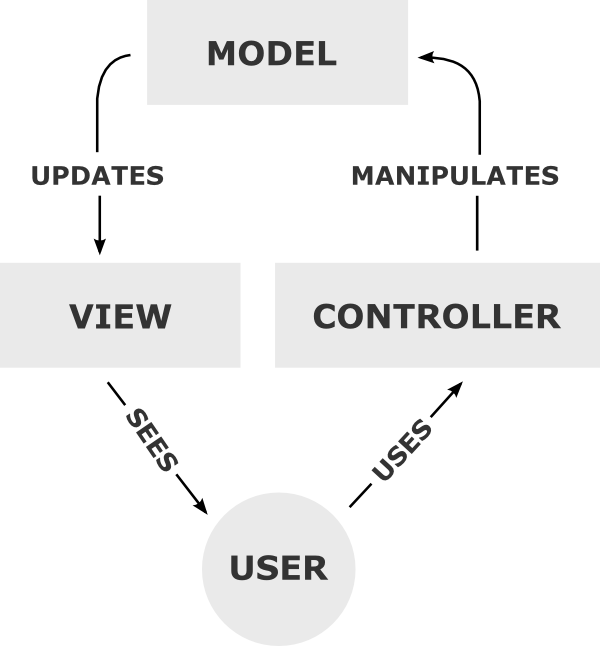
\includegraphics[width=0.38\textwidth]{images/Images/mvc.png}
	\end{center}
	\vspace{-20pt}
	\caption{MVC-mønsteret}
	\vspace{-20pt}
\end{wrapfigure}


Nedenfor beskriver vi de tre komponenter.

\textbf{Model}\\
De objekter, der udgør model-laget skal indeholde den før omtalte ''forretnings-logik'', samt alle data der skal modelleres i systemet.
Dataen, i form af objekter, gemmes oftest i en database eller fil, og er helt skjult for brugeren i den forstand, at al repræsentation af modellen foregår igennem view-delen af MVC-mønsteret.

\textbf{View}\\
Der er igennem forskellige views, at brugeren får præsenteret brugergrænsefladen - også kaldet UI(user-interface).
Derfor giver det også mening, at placere ''UI-logikken'' i denne del af MVC-mønsteret.
Typisk bliver et views indhold genereret ud fra data fra en model.
Et eksempel på dette ville være visning af en liste af objekter ud fra en model, der indeholder netop en liste.

\textbf{Controller}\\
Når det kommer til interaktionen mellem brugeren og systemet, er det controlleren der påtager sig opgaven.
Derfor er det også i de forskellige controllerere, at vi finder ''input-logikken''. Her bestemmes ud fra input fra brugeren hvilke data der skal arbejdes med i hvilken model og også hvilket view, der skal præsenteret for brugeren. Med dette kan vi også se, at viewet ikke indeholder nogenb logik og al manipulation af data altså foregår gennem controller komponenten.


\subsection{Program komponenter}\label{subsec:komp}

Der kan dannes forskellige komponenter i programmet ud fra de user stories der blev opgivet på \myref{sec:krav}.
Disse kan ses på figur \myref{figure:komp}.
Figuren viser hvordan de forskellige user stories kan deles op i komponenter, og hvordan disse komponenter afhænger og bruger hinanden som beskrevet ud fra vores user stories.

\begin{figure}

	\vspace{-20pt}
	\begin{center}
		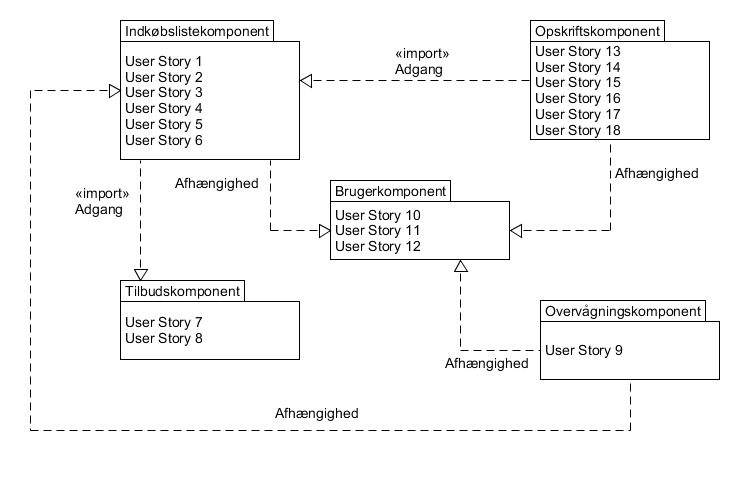
\includegraphics[scale=0.6]{images/Diagrams/Komponenter.png}
	\end{center}
	\vspace{-20pt}
	\caption{UML 2 Komponent diagram }
	\label{figure:komp}
	\vspace{-20pt}
\end{figure}

\textbf{Indkøbslistekomponentet} står for at lave indkøbslister, og tilføje varer og tilbud til disse.
Tilbudene skal importeres fra \textbf{tilbudskomponentet}, for at lave koblingen imellem varerne og tilbud.
Det er afhængigt af \textbf{brugerkomponentet} da indkøbslisterne hører til en bruger for at danne personlige lister. Brugerkomponentet er ansvarlig for alt der har med en bruger at gøre. Det indebærer at registrere hvem der er logget på, håndtere brugerens personlige indstillinger. Det er altså dette komponent der sørger for den personlige oplevelse på hjemmesiden.

\textbf{Opskriftskomponentet} er afhængig af brugerkomponentet, da det er brugerene i systemet der tilføjer opskrifter, samt giver opskrifterne en rating.
Dog er det opskriftskomponentet der står for dette, men det skal dog vide hvem der er logget ind på hjemmesiden.
Der er en adgang her fra til indkøbslisterne for at kunne tilføje ingredienser fra opskrifterne til indkøbslister.

\textbf{Overvågningskomponentet} står for at overvågningen af tilbud for en specifik varer kan foregå.
Der dannes en afhængighed herfra og til indkøbslistekomponentet da overvågningslisten gør brug af de metoder som der stilles til rådighed i dette komponenet, såsom tilføje varer, og finde tilbud.


\subsection{Klassediagram}
For at illustrere modellaget i vores MVC-mønster, har vi produceret et klassediagram (se \myref{diagram:klassediagram} nedenfor) i UML, der simplificerer strukturen.
Det skal bemærkes, at klasserne og felterne er på dansk i diagrammet, og på engelsk i selve koden af programmet. \fxfatal{Der er ingen adgangsting på dette, private, protected, public etc. Er det bevist? Derudover er det ikke klart hvilken datatype hvert felt er, også om det er en liste eller ej. - Troels - Fikser figuren senere - Søren}

\begin{figure}[H]
\centering
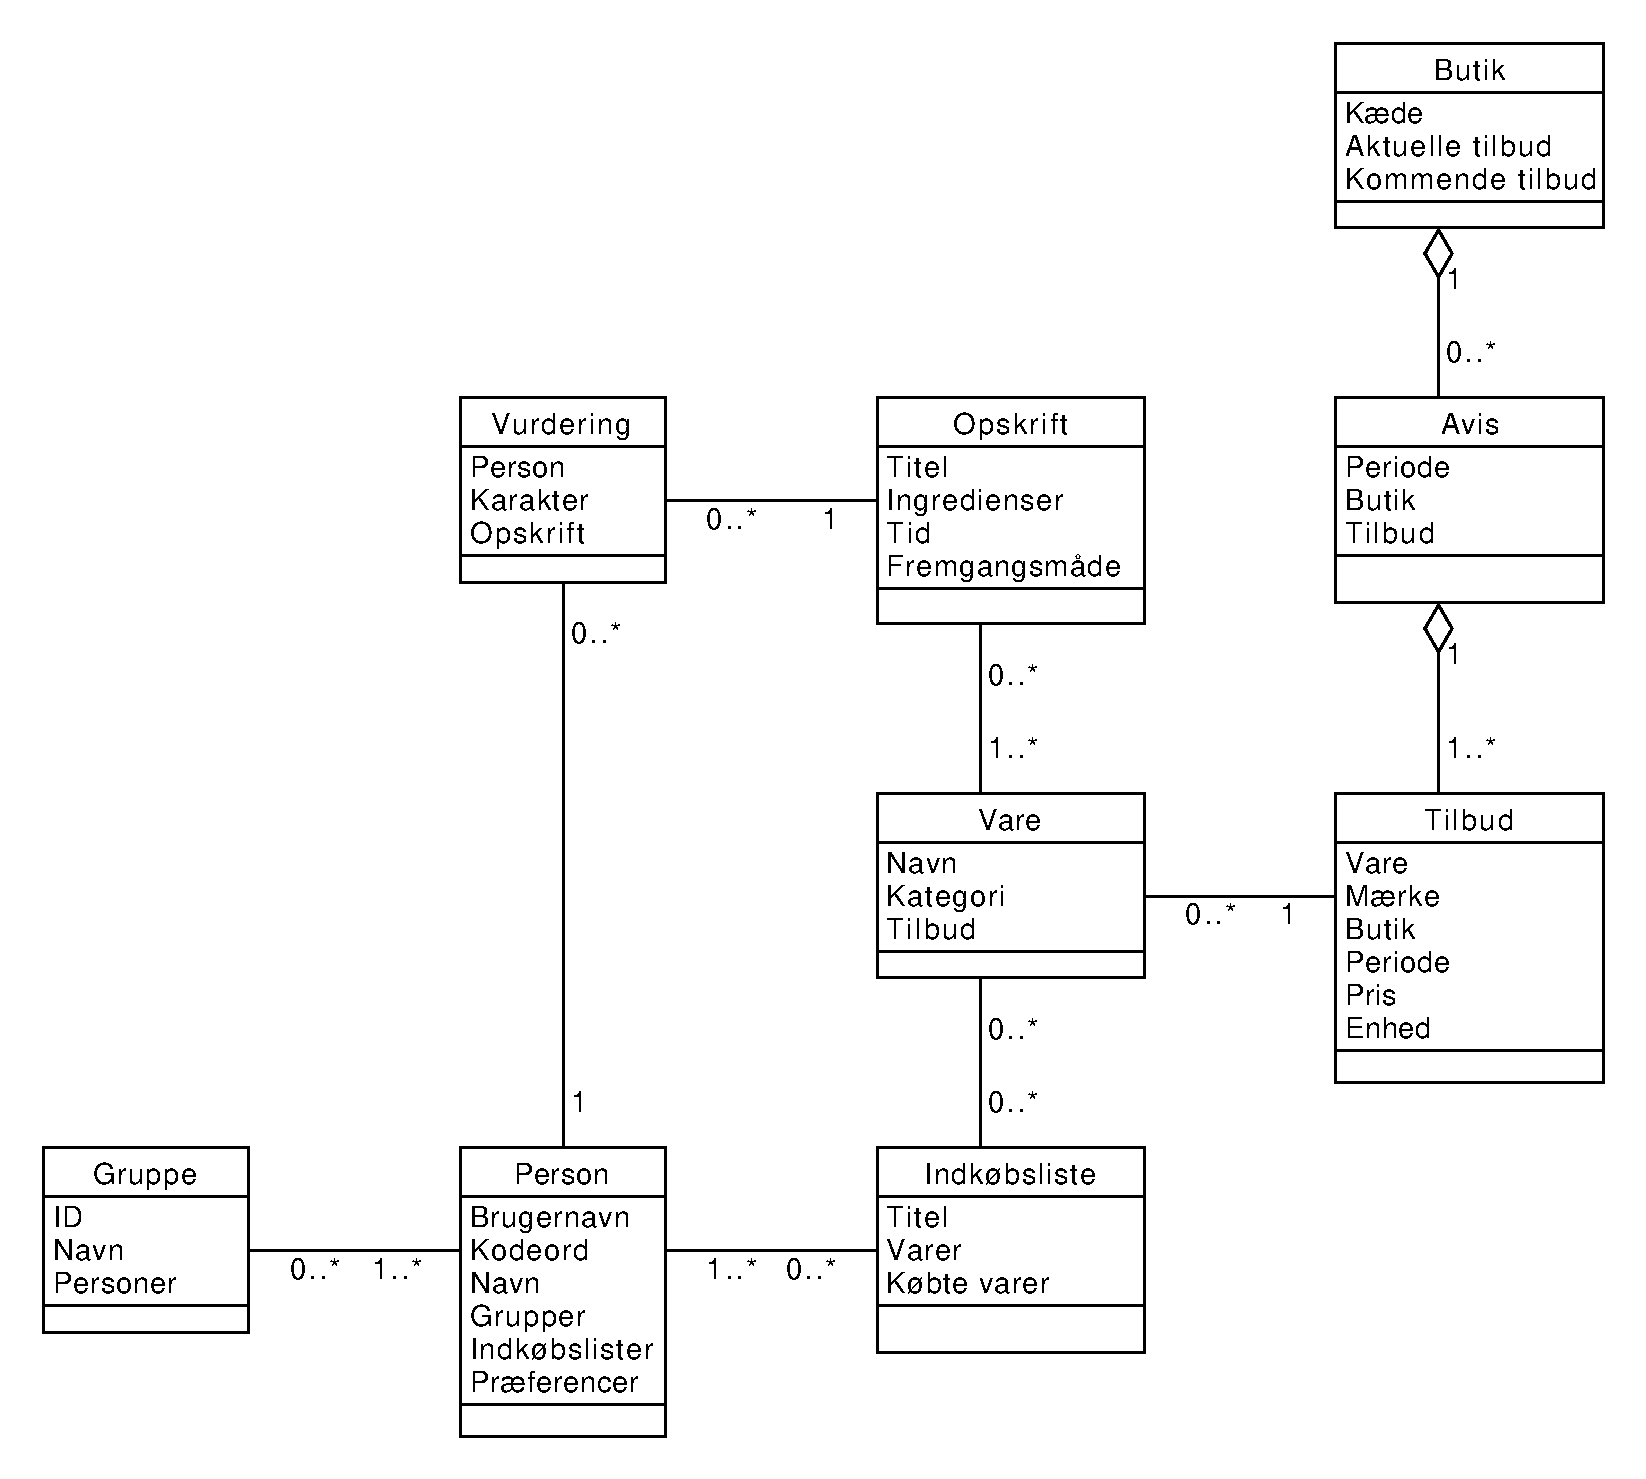
\includegraphics[width=0.8\linewidth]{/Diagrams/klassediagram_model_expanded_implemented.pdf}
\caption{UML klassediagram for modellaget i MVC-mønsteret}\label{diagram:klassediagram}
\end{figure}

\subsection{Klasserne}
Vi vil gennemgå klasserne, der optræder i klassediagrammet, og beskrive deres relationer samt deres felter.

\fxnote{Indsæt figur for hver enkelt klasse.}

\subsubsection{Person}
Person-klassen i modellen, er den der holder styr på brugeren og dennes basale attributter - herunder brugernavn, kodeord og kaldenavn.
Ydermere er det vigtigt, at objektet kan indeholde informationer om personens madpræferencer og vurderinger af opskrifter; dette er med til at give person-klassen en mere intim vinkel, og så at sige bedre afspejle den virkelige person, samt fungere som grundlag for anbefaling af opskrifter.
Det er naturligvis også vigtigt for et program, der omhandler bl.a. indkøbslister, at holde styr på en persons indkøbslister og lignende.
Til dette har person-klassen to felter der hedder henholdsvis, grupper og indkøbslister.
Begge felter er lister\fxfatal{Som nævnt tidligere er dette ikke klart fra diagrammet. - Troels}, der holder styr på personens relationer til netop grupper og indkøbslister - En person kan altså have relationer til flere grupper og flere indkøbslister, hvilket også kan ses ud fra de indtegnede relationer i klassediagrammet.


\subsubsection{Indkøbsliste}
Indkøbslister repræsenteres i systemet som klassen ´´Indkøbsliste'', og indeholder ID, titel og to lister med varer.
ID'et garanterer, at alle indkøbslister er unikke og kan skelnes fra hinanden på systemsiden.
Indkøbsliste-klassen har et titel felt, så brugeren også kan navigere mellem forskellige instanser.
De to lister af varer, holder styr på henholdsvis; varer som bliver tilføjet til listen, og varer som har været tilføjet men er blever markeret som købt.
Der er således kun styr på ''overstregede'' varer - altså dem der er købt, og ikke varer som bliver slettet fra listen.
En indkøbsliste kan godt eksisterer uden varer, idet brugeren skal kunne oprette lister, inden der er taget stilling til, hvilke varer der skal bruges.
Indkøbsliste har kun relation til en gruppe, men kan godt have relationer til flere personer.\fxnote{Findes der stadig to lister - Bruger vi dem ?}

\subsubsection{Vare}
Vare-klassen indeholder tre felter: Et navn på varen, som er generisk, for eksempel ''Letmælk'' og ''Cola'' istedet for ''Arla Letmælk'' og ''Pepsi''; en kategori, der beskriver varen, for eksempel ''Mejeri'' eller ''Pålæg''; og en liste over tilbud, der holder styr på, hvis og hvor varen eventuelt er på tilbud.
En vare behøver ikke være på en indkøbsliste eller opskrift for at eksistere \fixme{kan det passe?}, og kan have relationer til nul til mange tilbud.

\subsubsection{Tilbud}
Et tilbud som instans af Tilbud-klassen, indeholder felter der beskriver: Varen, mærket, hvilken butik tilbuddet befinder sig i, hvilken periode tilbuddet gælder i, prisen på tilbudet, og hvilken enhed/mængde tilbudet er i.
Ud fra disse atributter er det muligt at identificere tilbudet, og brugeren kan tage stilling til, om det er relevant.


\subsubsection{Opskrifter}
\lipsum[1]

\subsubsection{Vurdering}
\lipsum[1]

